\section{Requests}
\label{sec:requests}

A tensile force $F$ is applied to the end of the rod as shown in Figure \ref{fig:problem_representation}.

\begin{figure}[h]
    \centering
    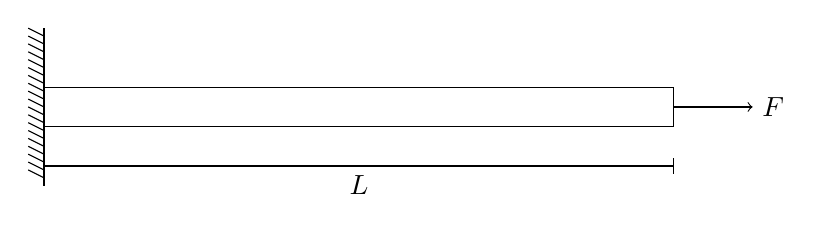
\begin{tikzpicture}[xscale=1, yscale=0.5]

        \draw (0,-0.5) rectangle (8, 0.5);
        \draw[->] (8, 0) -- ++(1, 0) node[right]{$F$};
        \draw[|-|] (0, -1.5) -- (8, -1.5) node[midway, below]{$L$};

        \draw (0, -2) -- (0,  2);

        \foreach \y in {-1.8, -1.6, ..., 1.8}
        \draw (0, \y) -- ++(-0.2, +0.2);


    \end{tikzpicture}
    \caption{Problem representation}
    \label{fig:problem_representation}
\end{figure}

Discretize the rod into five 4-node elements to compute the displacement of the rod throughout time.
Use an explicit integration scheme with Total Lagrangian finite element formulation.
Use the parent (element) system of coordinates.

Use a linear constitutive equation of the form $P = E \frac{du}{dX}$, where $P$ is the First Piola Kirchhoff stress.

The problem asks:

\begin{itemize}
    \item Write out the shape functions for the following 4-node element with total length $h_e$ and $\alpha = \beta = \frac{1}{3}$ in terms of the parent coordinate system, $-1 \leq \xi \leq 1$.
    \item Obtain the $B_0^e$ matrix for a general 4-node element and write the elemental force vectors $f_{int}^e$, $f_{ext}^e$, $f_{kin}^e$, and elemental mass matrix $M^e$ in discretized integral form. No need to integrate.
    \item Calculate the displacement of the node on the very right end after $t = 0.01s$ assuming the force is linearly increased at $100000 kN/s$ from $0 kN$ to $1000 kN$. Plot the deformation of the right end of the bar vs time. The force is intentionally high and rapid in order to allow for a visual representation of the deformation behavior (ignore yielding and assume elasticity).
    \item Is there a difference in the deformation behavior if the $1000 kN$ force is applied instantaneously at the beginning of the simulation (i.e. at $t=0$)? Plot the deformation of the right end vs time.
\end{itemize}

\begin{table}[H]
    \centering
    \begin{tabular}{|c|c|c|}
        \hline
        \textbf{Parameter} & \textbf{Value} & \textbf{Unit}                    \\ \hline
        $E_0$              & $70$           & $\text{GPa}$                     \\ \hline
        $\rho_0$           & $2700$         & $\text{kg/m\textsuperscript{3}}$ \\ \hline
        $A_0$              & $300$          & $\text{mm}^2$                    \\ \hline
        $L_0$              & $200$          & $\text{mm}$                      \\ \hline
    \end{tabular}
    \caption{Parameters of the rod element.}
    \label{tab:parameters_of_the_system}
\end{table}
